
\noindent\textbf{Dataset details.}
\label{sec:data}
We collect $11$ public RGB-D datasets, and over $8$ million data for training. It spreads over diverse indoor and outdoor scenes. Note that all datasets have provided %
camera intrinsic parameters. Apart from the test split of training datasets, we collect $7$ unseen datasets for robustness and generalization evaluation. Details of employed data are reported in the supplementary materials.  



\noindent\textbf{Implementation details.}
We employ an UNet architecture with the ConvNext-large~\cite{liu2022convnet} backbone. ImageNet-22K pre-trained weights are used for initialization. We use AdamW with a batch size of $192$, an initial learning rate $0.0001$ for all layers, and the polynomial decaying method with the power of $0.9$. We train our final model on $48$ A100 GPUs for $500$K iterations. Following the DiverseDepth~\cite{yin2021virtual}, we balance all datasets in a mini-batch to ensure each dataset accounts for an almost equal ratio. During training, images are processed by the canonical camera transformation module, flipped horizontally with a $50\%$ chance, and then randomly cropped into 
$512 \times 960$ pixels. For the ablation experiments, training settings are different as we sample $5000$ images from each dataset for training. We trained on $8$ GPUs for $150$K iterations.










\noindent\textbf{Evaluation details.}
a) To show the robustness of our metric depth estimation 
method, we test on 8 zero-shot benchmarks, including NYUv2~\cite{silberman2012indoor}, KITTI~\cite{Geiger2013IJRR}, NuScenes~\cite{caesar2020nuscenes}, 7-scenes~\cite{shotton2013scene}, iBIMS-1~\cite{koch2018evaluation}, DIODE~\cite{vasiljevic2019diode}, ETH3D~\cite{schops2017multi}. Following previous works~\cite{yuan2022new}, absolute relative error (AbsRel),  the accuracy under threshold ($\delta_{i} < 1.25^{i}, i=1, 2, 3$), root mean squared error (RMS), root mean squared error in log space (RMS\_{log}), and log10 error (log10) metrics are employed. 
b) Furthermore, %
we also follow current affine-invariant depth benchmarks~\cite{leres, zhang2022hierarchical} (Tab. \ref{Table: generalization evaluation.}) to evaluate the generalization ability on $5$ zero-shot datasets, \textit{i.e.},  NYUv2, DIODE, ETH3D, ScanNet~\cite{dai2017scannet}, and KITTI. We mainly compare with large-scale data trained models. Note that in this benchmark we follow existing methods to apply the scale shift alignment before evaluation. 
c) To evaluate our metric 3D reconstruction quality, we randomly sample 9 unseen scenes from NYUv2 and use colmap~\cite{schoenberger2016mvs} to obtain the camera poses for multi-frame reconstruction. Chamfer $l_1$ distance and the F-score~\cite{knapitsch2017tanks} are used to evaluate the reconstruction accuracy. 
d) In dense-SLAM experiments, following Li~\etal~\cite{li2021generalizing}, we test on the KITTI odometry benchmark~\cite{Geiger2013IJRR} and evaluate the average translational RMS drift ($\%, t_{rel}$) and rotational RMS drift ($\degree/100m, r_{rel}$) errors~\cite{Geiger2013IJRR}.
Note that all these depth and reconstruction evaluations use the same trained model. 

\subsection{Zero-shot Generalization %
Test
}

\begin{table}[!t]
\caption{Quantitative comparison on NYUv2 and KITTI benchmarks. Both datasets are unseen to our model, but we can achieve comparable performance with state-of-the-art methods.}
\vspace{-1 em}
\scalebox{0.67}{
\begin{tabular}{r |cccccc}
\toprule[1pt]
\multicolumn{7}{c}{\textbf{NYUv2 Benchmark}} \\ \hline
\multirow{1}{*}{Method} & $\boldsymbol{\delta_{1}}$$\uparrow$ & $\boldsymbol{\delta_{2}}$$\uparrow$ & $\boldsymbol{\delta_{3}}$$\uparrow$ & \textbf{AbsRel}$\downarrow$ & \textbf{log10}$\downarrow$ & \textbf{RMS}$\downarrow$  \\ \hline
Li \etal.~\cite{li2017two}               & $0.788$    & $0.958$    & $0.991$  & $0.143$   & $0.063$    & $0.635$     \\
Laina \etal.~\cite{laina2016deeper}      & $0.811$    & $0.953$    & $0.988$  & $0.127$   & $0.055$    & $0.573$       \\
VNL ~\cite{Yin2019enforcing}            & $0.875$   & $0.976$    & $0.994$  & $0.108$   & $0.048$    & $0.416$    \\ 
TrDepth~\cite{yang2021transformers}     & $0.900$   & $0.983$    & $0.996$  & $0.106$  & $0.045$     & $0.365$   \\
Adabins~\cite{bhat2021adabins}         & $0.903$    & ${0.984}$  & $\underline{0.997}$  & $0.103$  & $0.044$     & $0.364$    \\
NeWCRFs~\cite{yuan2022new}              
& ${0.922}$  & $\boldsymbol{0.992}$  & $\boldsymbol{0.998}$ 
& $0.095$  & $0.041$     & $\underline{0.334}$   \\ \hline
Ours CSTM\_image    
& $\boldsymbol{0.925}$  & $0.983$  & $0.994$ 
& $\underline{0.092}$   & $\underline{0.040}$   & ${0.341}$  \\
Ours CSTM\_label    
& $\underline{0.944}$  & $\underline{0.986}$  & $0.995$ 
& $\boldsymbol{0.083}$   & $\boldsymbol{0.035}$   & $\boldsymbol{0.310}$  \\\hline
\hline
\multicolumn{7}{c}{\textbf{KITTI Benchmark}} \\ \hline \hline
\multirow{1}{*}{Method} & $\boldsymbol{\delta_{1}}$$\uparrow$ & $\boldsymbol{\delta_{2}}$$\uparrow$ & $\boldsymbol{\delta_{3}}$$\uparrow$ & \textbf{AbsRel} $\downarrow$ & \textbf{RMS} $\downarrow$ & \textbf{RMS\_log} $\downarrow$ \\ \hline
Guo \etal \cite{guo2018learning}  & $0.902$  & $0.969$  & $0.986$ & $0.090$ & $3.258$ & $0.168$    \\
VNL~\cite{Yin2019enforcing} & ${0.938}$   & ${0.990}$   & ${0.998}$  & ${0.072}$  & $3.258$      & ${0.117}$    \\ 
TrDepth~\cite{yang2021transformers}   & $0.956$  & $0.994$  & $0.999$   & $0.064$  & $2.755$  & $0.098$  \\
Adabins~\cite{bhat2021adabins} & $0.964$  & $0.995$  & $0.999$   & $\underline{0.058}$  & $2.360$  & $0.088$  \\
NeWCRFs~\cite{yuan2022new} 
& $\boldsymbol{0.974}$  & $\boldsymbol{0.997}$  & $\underline{0.999}$   & $\boldsymbol{0.052}$  & $\boldsymbol{2.129}$  & $\boldsymbol{0.079}$  \\ \hline
Ours CSTM\_image & 
$\underline{0.967}$   & $\underline{0.995}$   & $\boldsymbol{0.999}$  
& $0.060$  & ${2.843}$     & $\underline{0.087}$    \\ 
Ours CSTM\_label 
& ${0.964}$   & ${0.993}$   & ${0.998}$  
& $0.058$  & ${2.770}$     & ${0.092}$    \\ \hline
\toprule[1pt]
\end{tabular}\newline}
\label{table:errors cmp on NYUD-V2}
\vspace{-2 em}
\end{table}






\begin{table*}[]
\renewcommand\arraystretch{1.1}
\caption{Quantitative comparison of 3D scene reconstruction with LeReS~\cite{leres}, DPT~\cite{ranftl2021vision}, %
RCVD~\cite{kopf2021rcvd}, 
SC-DepthV2~\cite{bian2021tpami}, and a learning-based MVS method (DPSNet~\cite{im2019dpsnet}) on 9 unseen NYUv2 scenes. Apart from DPSNet and ours, other methods have to align the scale with ground truth depth for each frame. As a result, our reconstructed 3D scenes achieve the best performance.}
\vspace{-1 em}
\centering
\resizebox{.98\linewidth}{!}{%
  \centering
  \small 
  \setlength{\tabcolsep}{0.5mm}{\begin{tabular}{@{} r |rc|rc|rc|rc|rc|rc|rc|rc|rc@{}}
    \toprule
    \multirow{2}{*}{Method} & \multicolumn{2}{c|}{Basement\_0001a} & \multicolumn{2}{c|}{Bedroom\_0015} & \multicolumn{2}{c|}{Dining\_room\_0004} & \multicolumn{2}{c|}{Kitchen\_0008} & \multicolumn{2}{c|}{Classroom\_0004} & \multicolumn{2}{c|}{Playroom\_0002}  & \multicolumn{2}{c|}{Office\_0024} & \multicolumn{2}{c|}{Office\_0004} & \multicolumn{2}{c}{Dining\_room\_0033}\\
      & C-$l_1$$\downarrow$ & F-score $\uparrow$ & C-$l_1$$\downarrow$ & F-score $\uparrow$ & C-$l_1$$\downarrow$ & F-score $\uparrow$ & C-$l_1$$\downarrow$ & F-score $\uparrow$ & C-$l_1$$\downarrow$ & F-score $\uparrow$ & C-$l_1$$\downarrow$ & F-score $\uparrow$ &
      C-$l_1$$\downarrow$ & F-score $\uparrow$ & C-$l_1$$\downarrow$ & F-score $\uparrow$ & C-$l_1$$\downarrow$ & F-score $\uparrow$\\ \hline
    RCVD~\cite{kopf2021rcvd} & 0.364 & 0.276 
            & 0.074 & 0.582 &
             0.462 & 0.251 &
             0.053 & 0.620 &
              0.187 & 0.327 &
             0.791 & 0.187 &
             0.324 & 0.241  &
             0.646 & 0.217 &
             0.445 & 0.253 \\

    SC-DepthV2~\cite{bian2021tpami}  & 0.254 & 0.275 &
             0.064 & 0.547 &
             0.749 & 0.229 &
             0.049 & 0.624 &
              0.167 & 0.267 &
             0.426 & 0.263 &
             0.482 & 0.138  &
             0.516 & 0.244 &
             0.356 &0.247 \\

    DPSNet~\cite{im2019dpsnet} & 0.243 & 0.299 &
             0.195 & 0.276 &
             0.995 & 0.186 &
             0.269 & 0.203 &
             0.296 & 0.195 &
             0.141 & 0.485 &
             0.199 & 0.362  &
             0.210 & 0.462 &
             0.222 & 0.493 \\
              
    DPT~\cite{leres} & 0.698 & 0.251 &
             0.289 & 0.226 &
             0.396 & 0.364 &
             0.126 & 0.388 &
             0.780 & 0.193 & 
             0.605 & 0.269 &
             0.454 & 0.245  &
             0.364 & 0.279 &
             0.751 & 0.185 \\  
    LeReS~\cite{leres} & 0.081 & 0.555 &
             0.064 & 0.616 &
             0.278 & 0.427 &
             0.147 & 0.289 &
             \textbf{0.143} & \textbf{0.480} &
             0.145 & 0.503 &
             0.408 & 0.176  &
             0.096 & 0.497 &
             0.241 & 0.325 \\  \hline
    Ours & \textbf{0.042} & \textbf{0.736} &
             \textbf{0.059} & \textbf{0.610} &
             \textbf{0.159} & \textbf{0.485} &
             \textbf{0.050} & \textbf{0.645} &
             0.145 & 0.445 &
             \textbf{0.036} & \textbf{0.814} &
             \textbf{0.069} & \textbf{0.638}  &
             \textbf{0.045} & \textbf{0.700} &
             \textbf{0.060} & \textbf{0.663} \\

    \bottomrule
  \end{tabular}}}
  \label{tab: NYUD reconstruction cmp.}
\end{table*}

\begin{figure*}[]
\centering
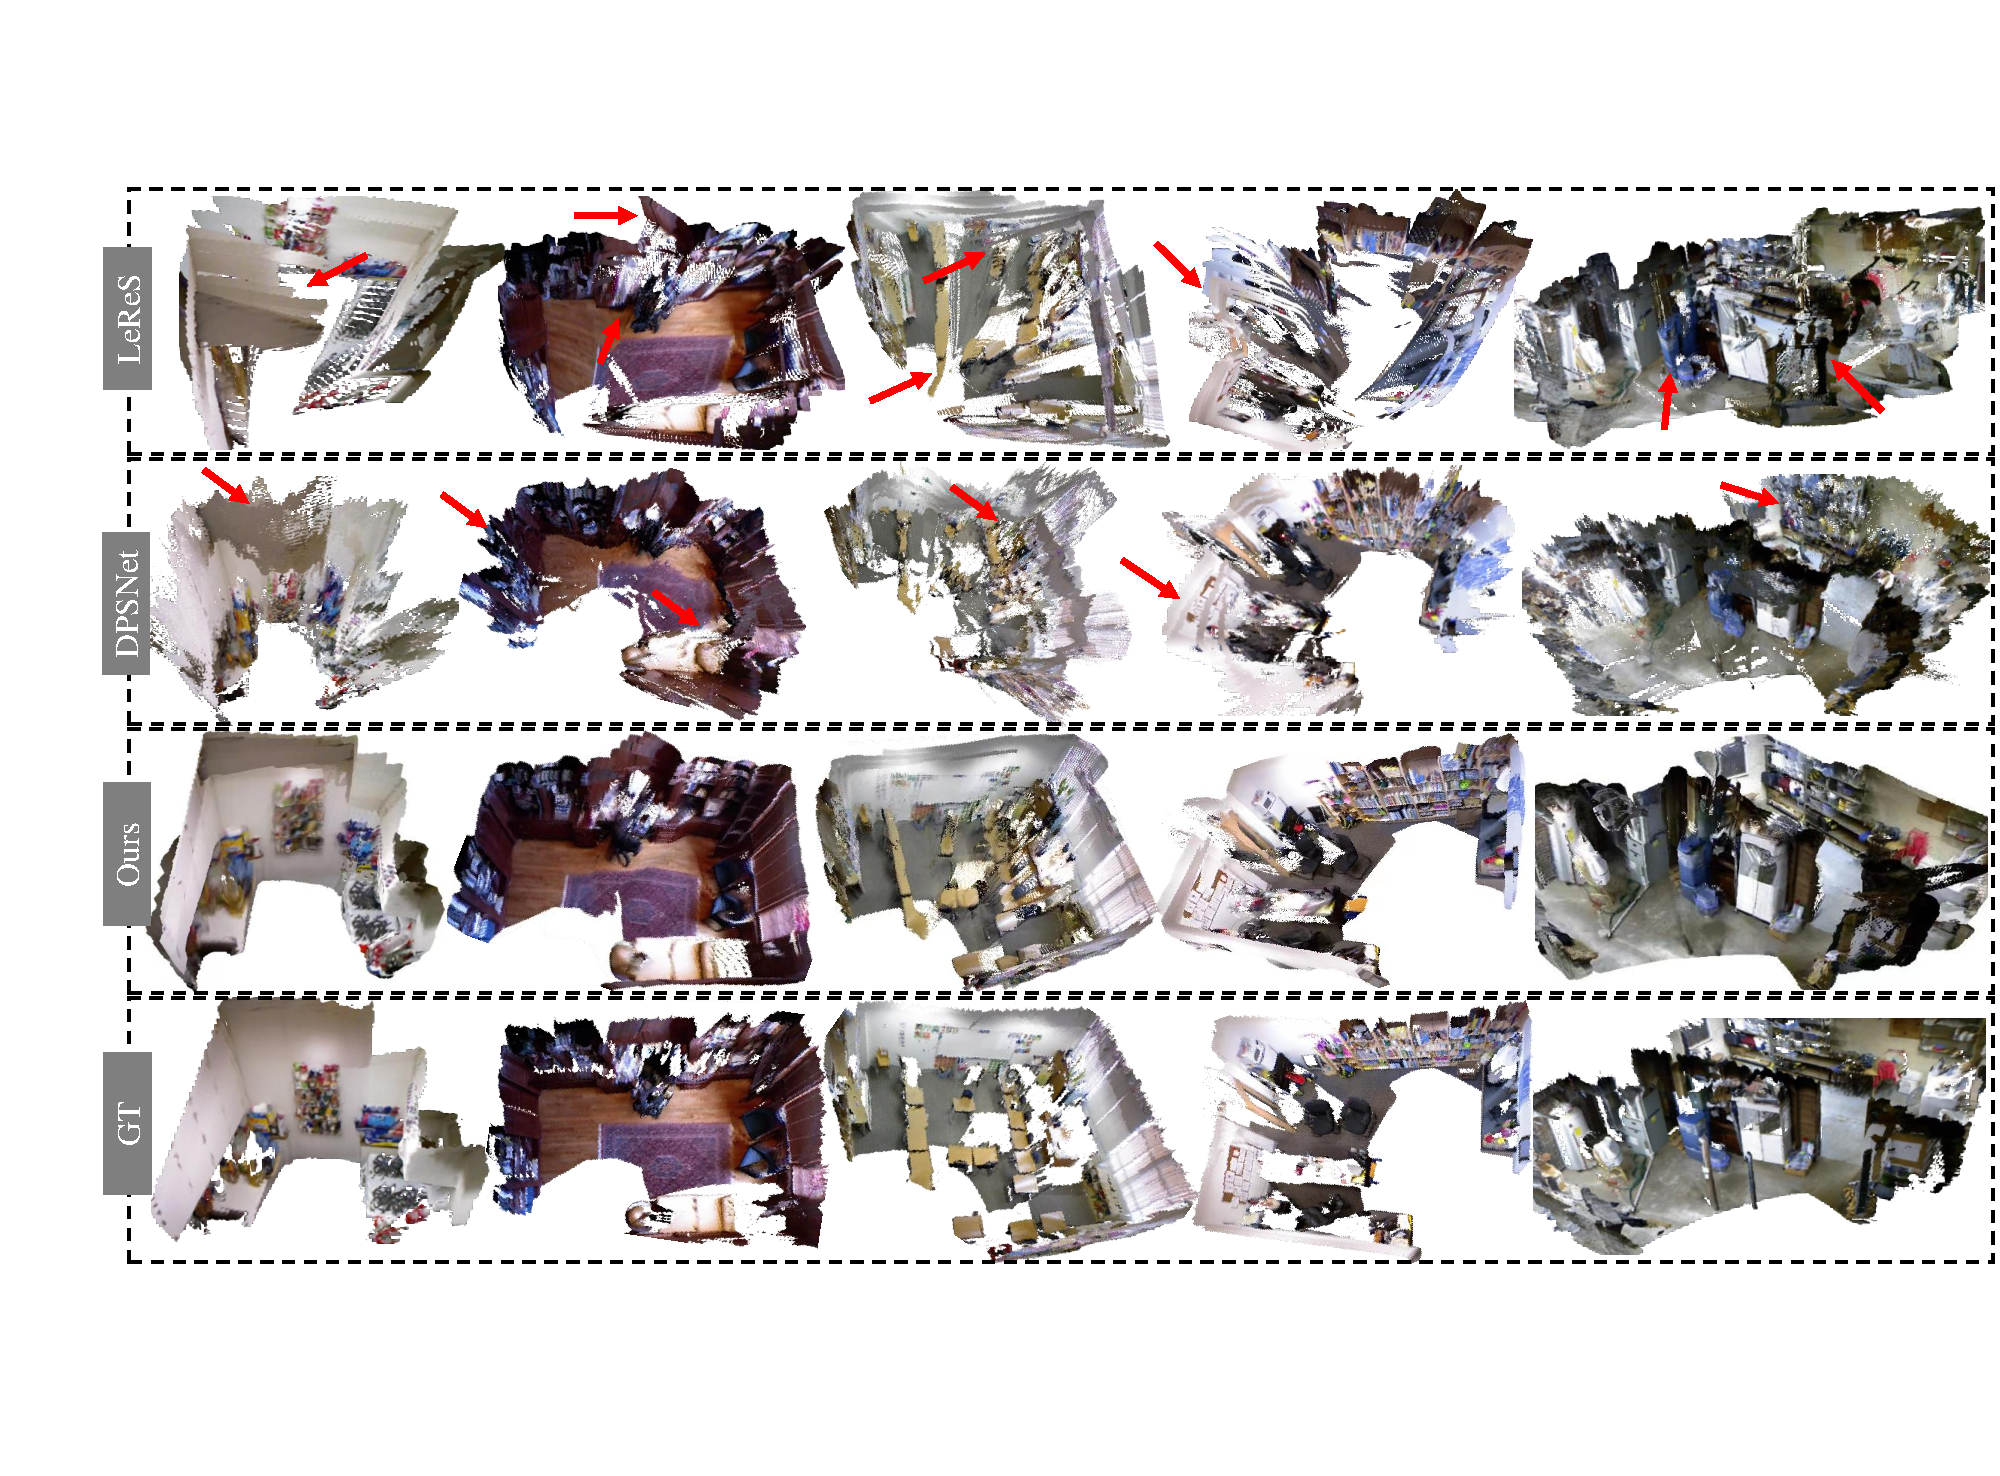
\includegraphics[width=0.95\textwidth]{./files/3dreconstruction.pdf}
\vspace{-1 em}
\caption{\textbf{Reconstruction of zero-shot scenes with multiple views.} We sample several NYUv2 scenes for 3D reconstruction comparison. As our method can predict accurate metric depth, thus all frame's predictions are  fused together for scene reconstruction. By contrast, LeReS~\cite{leres}'s depth is up to an unknown scale and shift, which causes noticeable distortions. DPSNet~\cite{im2019dpsnet} is a multi-view stereo method, which cannot work well on low-texture regions. }
\label{fig: visual nyud reconstruction cmp.}
\vspace{-1em}
\end{figure*}




\noindent\textbf{Evaluation on metric depth benchmarks.} To evaluate the accuracy of predicted metric depth, firstly,  we compare with state-of-the-art (SOTA) metric depth prediction methods on NYUv2~\cite{silberman2012indoor}, KITTI~\cite{geiger2012we}.
We use the same model to do %
all evaluations. %
Results are reported in Tab.~\ref{table:errors cmp on NYUD-V2}. Without any fine-tuning or metric adjustment,  we can achieve comparable performance with SOTA methods, which are trained on benchmarks for hundreds of epochs. %







Furthermore, We collect $6$ unseen datasets to do more metric accuracy evaluation. These datasets contain a wide range of indoor and outdoor scenes, including rooms, buildings, and driving scenes. The camera models are also various, e.g. 7scenes has a short focal length (around 500), while ETH3D is 2000. We mainly compare with the SOTA metric depth estimation methods and take their NYUv2 and KITTI models for indoor and outdoor scenes evaluation respectively. From Tab. \ref{table: metric eval on more datasets.}, we observe that although 7Scenes is similar to NYUv2 and NuScenes is similar to KITTI, existing methods face a noticeable performance decrease. In contrast, our model is more robust. %

\begin{table*}[]
\centering
 \caption{Quantitative comparison with SOTA metric depth methods on $6$ unseen benchmarks. For SOTA methods, we use their NYUv2 and KITTI models for indoor and outdoor scenes evaluation respectively, while we use the same model for all zero-shot testing. }
 \vspace{-1 em}
 \resizebox{0.9\linewidth}{!}{%
\begin{tabular}{l|lll|lll}
\toprule[1pt]
\multirow{2}{*}{Method}        & DIODE(Indoor) & iBIMS-1 & 7Scenes      & DIODE(Outdoor)      & ETH3D      & NuScenes     \\
        & \multicolumn{3}{c|}{Indoor scenes (AbsRel$\downarrow$/RMS$\downarrow$)}  & \multicolumn{3}{c}{Outdoor scenes (AbsRel$\downarrow$/RMS$\downarrow$)} \\ \hline
Adabins~\cite{bhat2021adabins}  
         &  0.443 / 1.963       
         &0.212 / 0.901         
         & 0.218 / 0.428 
         &0.865 / 10.35                     
         &1.271 / 6.178            
         &0.445 / 10.658              \\
NewCRFs~\cite{yuan2022new}  
         &0.404 / 1.867               
         &0.206 / 0.861         
         &0.240 / 0.451 
         &0.854 / 9.228                     
         &0.890 / 5.011            
         &0.400 / 12.139              \\ \hline
Ours\_CSTM\_label    
        &\textbf{0.252} / \underline{1.440}               
        & \underline{0.160} / \textbf{0.521}         
        &  \textbf{0.183} / \textbf{0.363}   
        &\textbf{0.414} / \underline{6.934}                     
        & \underline{0.416} / \underline{3.017}          
        & \underline{0.154} / \underline{7.097}             \\
Ours\_CSTM\_image    
        & \underline{0.268} / \textbf{1.429}         
        & \textbf{0.144} / \underline{0.646}        
        & \underline{0.189} / \underline{0.388}  
        & \underline{0.535} / \textbf{6.507}                    
        & \textbf{0.342} / \textbf{2.965}           
        & \textbf{0.147} / \textbf{5.889}    \\ \toprule[1pt]
\end{tabular}}
\label{table: metric eval on more datasets.}
\vspace{-1 em}
\end{table*}










\begin{table*}[t]
\centering
\caption{
Comparison with SOTA affine-invariant depth methods on 5 zero-shot transfer benchmarks.
Our model significantly outperforms previous methods and sets new state-of-the-art. Following the benchmark setting, all methods have manually aligned the scale and shift. 
}
\vspace{-1 em}
\setlength{\tabcolsep}{2pt}
\resizebox{0.99\linewidth}{!}{%
\begin{tabular}{ r |ll|ll|ll|ll|ll|ll|l}
\toprule[1pt]
\multirow{2}{*}{Method} & \multirow{2}{*}{Backbone} & \multirow{2}{*}{\#Params} & \multicolumn{2}{c|}{NYUv2} & \multicolumn{2}{c|}{KITTI} & \multicolumn{2}{c|}{DIODE} & \multicolumn{2}{c|}{ScanNet} & \multicolumn{2}{c|}{ETH3D}  & \multicolumn{1}{c}{Rank} \\
&  &   & AbsRel$\downarrow$     & $\delta_{1}$$\uparrow$     & AbsRel$\downarrow$      & $\delta_{1}$$\uparrow$      & AbsRel$\downarrow$      & $\delta_{1}$$\uparrow$      &AbsRel$\downarrow$      & $\delta_{1}$$\uparrow$       &AbsRel$\downarrow$     & $\delta_{1}$$\uparrow$  & \\ \hline
DiverseDepth~\cite{yin2021virtual}& ResNeXt50~\cite{xie2017aggregated}& 25M  
&$0.117$ &$0.875$ 
&$0.190$ &$0.704$ 
&$0.376$ &$0.631$ 
&$0.108$ &$0.882$ 
&$0.228$ &$0.694$  & $7.7$ \\
MiDaS~\cite{Ranftl2020}& ResNeXt101&  88M %
&$0.111$ &$0.885$ 
&$0.236$ &$0.630$ 
&$0.332$ &$0.715$ 
&$0.111$ &$0.886$  
& $0.184$ &$0.752$ & $7.2$ \\
Leres~\cite{leres} & ResNeXt101&  %
&$0.090$  &${0.916}$  
&${0.149}$ &${0.784}$ 
&${0.271}$ &${0.766}$ 
&${0.095}$ &${0.912}$ 
&${0.171}$ &${0.777}$ & $5.4$ \\
Omnidata~\cite{eftekhar2021omnidata} & ViT-base& %
& 0.074 & 0.945 
& 0.149 & 0.835
& 0.339 & 0.742 
& 0.077 & 0.935 
& 0.166 & 0.778 & $4.9$ \\
HDN~\cite{zhang2022hierarchical} & ViT-Large~\cite{dosovitskiy2020an}&  306M  
&$0.069$  &$0.948$  
&$0.115$ &$0.867$ 
&$0.246$ &$0.780$ 
&$0.080$ &$0.939$ 
&$0.121$ &$0.833$ & $3.7$ \\
DPT-large~\cite{ranftl2021vision} & ViT-Large& %
& 0.098 & 0.903 
& 0.10 & 0.901
& \textbf{0.182} & 0.758 
& 0.078 & 0.938 
& 0.078 & 0.946 & $3.8$ \\
\hline
Ours CSTM\_image & ConvNeXt-large~\cite{liu2022convnet}&  198M 
&$\underline{0.058}$  &$\underline{0.963}$  
&$\textbf{0.053}$ &$\underline{0.965}$ 
&$\underline{0.211}$ &$\textbf{0.825}$ 
&$\textbf{0.074}$ &$\textbf{0.942}$ 
&$\textbf{0.064}$ &$\textbf{0.965}$ & $1.3$ \\ 
Ours CSTM\_label & ConvNeXt-large&   
&$\textbf{0.050}$  &$\textbf{0.966}$  
&$\underline{0.058}$ &$\textbf{0.970}$ 
&$0.224$ &$\underline{0.805}$ 
&$\textbf{0.074}$ &$\underline{0.941}$ 
&$\underline{0.066}$ &$\underline{0.964}$ & $1.8$ \\

 \toprule[1pt]
\end{tabular}}

\label{Table: generalization evaluation.}
\vspace{-1.5em}
\end{table*}

\noindent\textbf{Generalization over diverse scenes.}
Affine-invariant depth benchmarks decouple the scale's effect, which aims to evaluate the model's generalization ability to diverse scenes. Recent impact works, such as MiDaS, LeReS, and DPT, achieved promising performance on them. Following them, we test on 5 datasets and manually align the scale and shift to the ground-truth depth before evaluation. Results are reported in Tab.~\ref{Table: generalization evaluation.}. Although our method enforces the network to recover more challenging metric information, our method outperforms them by a large margin on most datasets. 



\begin{figure}[!bth]
\centering
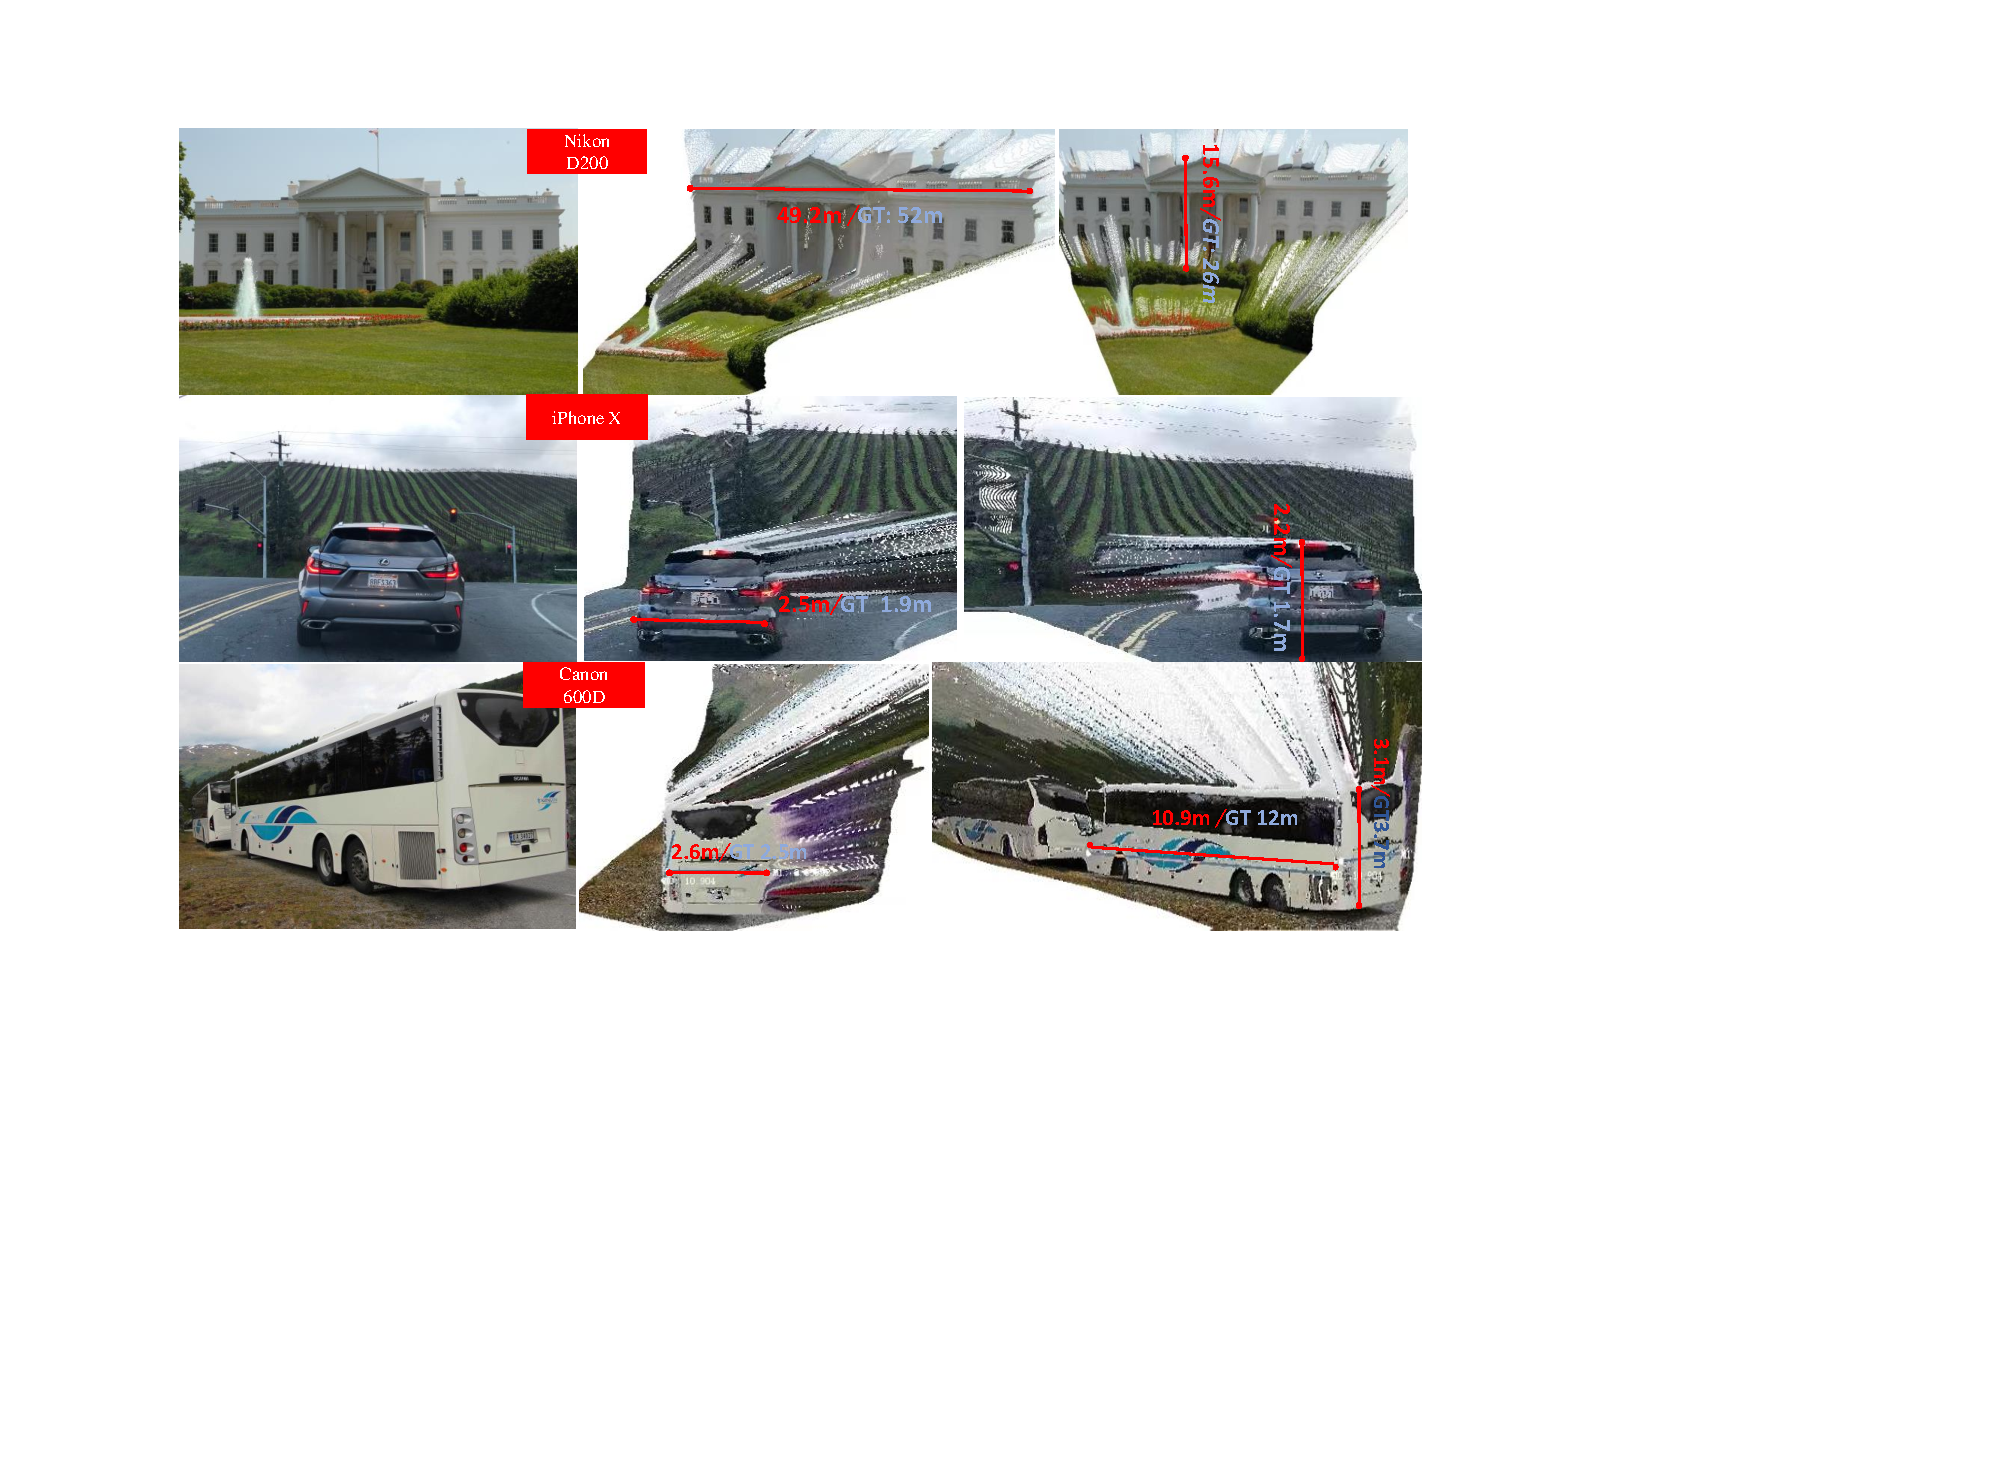
\includegraphics[width=0.5\textwidth]{./files/metrology_in_the_wild.pdf}
\vspace{-2 em}
\caption{\textbf{Reconstruction of in-the-wild scenes.} We collect several Flickr photos, which are captured by various cameras. With photos' metadata, we reconstruct the 3D metric shape and measure structures' sizes. Red and blue marks are ours and ground-truth sizes respectively. }
\label{fig: reconstruction in the wild.}
\vspace{-1em}
\end{figure}


\subsection{Applications Based on Our Method}
In these experiments, we apply the CSTM\_image model to various tasks. 

\noindent\textbf{3D scene reconstruction .}
To demonstrate our work can recover the 3D metric shape in the wild, we first do the quantitative comparison on 9 NYUv2 scenes, which are unseen during training. We predict the per-frame metric depth and then fuse them together with provided camera poses. Results are reported in Tab. \ref{tab: NYUD reconstruction cmp.}. We compare with the video consistent depth prediction method (RCVD~\cite{kopf2021rcvd}), the unsupervised video depth estimation method (SC-DepthV2~\cite{bian2021tpami}), the 3D scene shape recovery method (LeReS~\cite{leres}), affine-invariant depth estimation method (DPT~\cite{ranftl2021vision}), and the multi-view stereo reconstruction method (DPSNet~\cite{im2019dpsnet}). Apart from DPSNet and our method, other methods have to align the scale with the ground truth depth for each frame. Although our method does not aim for the video or multi-view reconstruction problem, our method can achieve promising consistency between frames and reconstruct much more accurate 3D scenes than others on these zero-shot scenes.  From the qualitative comparison in Fig.~\ref{fig: visual nyud reconstruction cmp.}. our reconstructions have much less noise and outliers. 

\noindent\textbf{Dense-SLAM mapping.}
Monocular SLAM is an important robotics application. It only relies on a monocular video input to create the trajectory and dense 3D mapping. Owing to limited photometric and geometric constraints, existing methods face serious scale drift problems in large scenes and cannot recover the metric information. Our robust metric depth estimation method is a strong depth prior to the SLAM system. To demonstrate this benefit,  we naively input our metric depth to the SOTA SLAM system, Droid-SLAM~\cite{teed2021droid}, and evaluate the trajectory on KITTI. We do not do any tuning on the original system. Trajectory comparisons are reported in Tab. \ref{tab: KITTI SLAM.}. As Droid-SLAM can access accurate per-frame metric depth, like an RGB-D SLAM, the translation drift ($t_{rel}$) decreases significantly. Furthermore, with our depths, Droid-SLAM can perform denser and more accurate 3D mapping. An example is shown in Fig.~\ref{Fig: first page fig.} and more cases are shown in the supplementary materials.   

We also test on the ETH3D SLAM benchmarks. Results are reported in Tab.~\ref{Tab: ETH3D SLAM}. Droid with our depths has much better SLAM performance. As the ETH3D scenes are all small-scale indoor scenes, the performance improvement is less than that on KITTI. 

\begin{table}[]
\renewcommand\arraystretch{1.1}
\caption{Comparison with SOTA SLAM methods on KITTI. We input predicted metric depth to the Droid-SLAM~\cite{teed2021droid} (`Droid+Ours'), which outperforms others by a large margin on trajectory accuracy.}
\centering
\resizebox{.98\linewidth}{!}{%
  \centering
  \small 
  \setlength{\tabcolsep}{0.5mm}{\begin{tabular}{@{} l |c|c|c|c|c|c|c@{}}
    \toprule
    \multirow{2}{*}{Method} & Seq 00 & Seq 02 & Seq 05 & Seq 06 & Seq 08 & Seq 09 & Seq 10 \\ \cline{2-8} 
      & \multicolumn{7}{c}{Translational RMS drift ($t_{rel}, \downarrow$) / Rotational RMS drift ($r_{rel}, \downarrow$)} \\ \hline
    GeoNet~\cite{yin2018geonet} & 27.6/5.72 & 42.24/6.14 & 
             20.12/7.67 & 
             9.28/4.34 & 
             18.59/7.85 & 
             23.94/9.81 & 
             20.73/9.1  \\
    VISO2-M~\cite{song2015high}  & 12.66/2.73 & 
             9.47/1.19 & 
             15.1/3.65 & 
             6.8/1.93 & 
             14.82/2.52 & 
             3.69/1.25 & 
             21.01/3.26  \\

    ORB-V2~\cite{murORB2} & 11.43/0.58 & 
             10.34/0.26 &
             9.04/0.26 & 
             14.56/0.26 & 
             11.46/0.28 & 
             9.3/0.26 & 
             2.57/0.32    \\
              
    Droid~\cite{teed2021droid} & 33.9/\textbf{0.29} & 
             34.88/\textbf{0.27} & 
             23.4/0.27 & 
             17.2/0.26 & 
             39.6/0.31 & 
             21.7/0.23 & 
             7/0.25   \\  \hline
             
    Droid+Ours & \textbf{1.44}/0.37 & 
             \textbf{2.64}/0.29 & 
             \textbf{1.44}/\textbf{0.25} & 
             \textbf{0.6}/\textbf{0.2} & 
             \textbf{2.2}/\textbf{0.3} & 
             \textbf{1.63}/\textbf{0.22} & 
             \textbf{2.73}/\textbf{0.23}    \\

    \bottomrule
  \end{tabular}}}
  \label{tab: KITTI SLAM.}
\end{table}

\begin{table}[t]
\caption{
Comparison of VO error on ETH3D benchmark. Droid SLAM system is input with our depth (`Droid + Ours'), and ground-truth depth (`Droid + GT'). The average trajectory error is reported.
}
 \resizebox{\linewidth}{!}{%
\begin{tabular}{l|llllll}
\hline
             & Einstein\_global & Manquin4 & Motion1 & Plantscene3 & sfm\_house\_loop & sfm\_lab\_room2 \\ \hline
& \multicolumn{6}{c}{Average trajectory error ($\downarrow$)}  \\ \hline
Droid        & 4.7                               & 0.88     & 0.83    & 0.78        & 5.64             & 0.55            \\ 
%Droid+LeReS  & 7.8                               & 0.91     & 0.95    & 0.80        & 6.9              & 0.55            \\ \hline
Droid + Ours & 1.5                               & 0.69     & 0.62    & 0.34        & 4.03             & 0.53            \\ 
Droid + GT   & 0.7                               & 0.006    & 0.024   & 0.006       & 0.96             & 0.013           \\ \hline
\end{tabular}}
\label{Tab: ETH3D SLAM}
\vspace{-1 em}
\end{table}

\noindent\textbf{Metrology in the wild.} To show the robustness and accuracy of our recovered metric 3D, we download Flickr photos captured by various cameras and collect coarse camera intrinsic parameters from their metadata. We use our CSTM\_image model to reconstruct their metric shape and measure structures' sizes (marked in red in Fig.~\ref{fig: reconstruction in the wild.}), while the ground-truth sizes are in blue. It shows that our measured sizes are very close to the ground-truth sizes. 






\subsection{Ablation Study}
\noindent\textbf{Ablation on canonical transformation.}
We study the effect of our proposed canonical transformation for the input images (`CSTM\_input') and the canonical transformation for the ground-truth labels (`CSTM\_output'). Results are reported in  Tab. \ref{table: importance of camera model.}. We train the model on sampled mixed data (55K images) and test it on 6 datasets. A naive baseline (`Ours w/o CSTM') is to remove CSTM modules and enforce the same supervision as ours. Without CSTM, the model is unable to converge when training on mixed metric datasets and cannot achieve metric prediction ability on zero-shot datasets. This is why recent mixed-data training methods compromise learning the affine-invariant depth to avoid metric issues. In contrast, our two CSTM methods both can enable the model to achieve the metric prediction ability, and they can achieve comparable performance. Tab. \ref{table:errors cmp on NYUD-V2} also shows comparable performance. Therefore, both adjusting the supervision and the input image appearance during training can solve the metric ambiguity issues. Furthermore, we compare with CamConvs~\cite{facil2019cam}, which encodes the camera model in the decoder with a 4-channel feature. `CamConvs' employ the same training schedule, model, and training data as ours. This method enforces the network to implicitly understand various camera models from the image appearance and then bridges the imaging size to the real-world size. We believe that this method challenges the data diversity and network capacity, thus their performance is worse than ours. 


\begin{table}[]
\caption{Effectiveness of our CSTM. CamConvs~\cite{facil2019cam} directly encodes various camera models in the network, while we perform a simple yet effective transformation to solve the metric ambiguity. Without CSTM, the model cannot achieve transferable metric prediction ability.}
\vspace{-1 em}
\scalebox{0.65}{
\begin{tabular}{l|lll|lll}
\toprule[1pt]
\multirow{2}{*}{Method}        & DDAD & Lyft & DS & NS & KITTI & NYU \\ 
        &\multicolumn{3}{c|}{Test set of train. data (AbsRel$\downarrow$)}     & \multicolumn{3}{c}{Zero-shot test set (AbsRel$\downarrow$)} \\  \hline 
w/o CSTM &$0.530$ &$0.582$  &$0.394$  &$1.00$ & $0.568$      &$0.584$  \\
CamConvs~\cite{facil2019cam}  &$0.295$ &$0.315$  &$0.213$ &$0.423$  &$0.178$      &$0.333$   \\
Ours CSTM\_image &$0.190$ &$0.235$  &$0.182$  &$0.197$ & $0.097$      &$0.210$ \\
Ours CSTM\_label &$0.183$ &$0.221$  &$0.201$  &$0.213$ & $0.081$      &$0.212$  \\
\toprule[1pt]
\end{tabular}}
\label{table: importance of camera model.}
\vspace{-1 em}
\end{table}





\noindent\textbf{Ablation on canonical space.}
We study the effect of the canonical camera here, \textit{i.e.}, the canonical focal length. We train the model on the small sampled dataset and test it on the validation set of training data and testing data. The average AbsRel error is calculated.  We experiment on 3 different focal lengths, \ie, 500, 1000, 1500. Experiments show that $focal=1000$ has slightly better performance than others, see Fig.~\ref{fig: canonical focal length.} for details. Thus we set the canonical focal length to 1000 in our experiments.

\begin{figure}[]
\centering
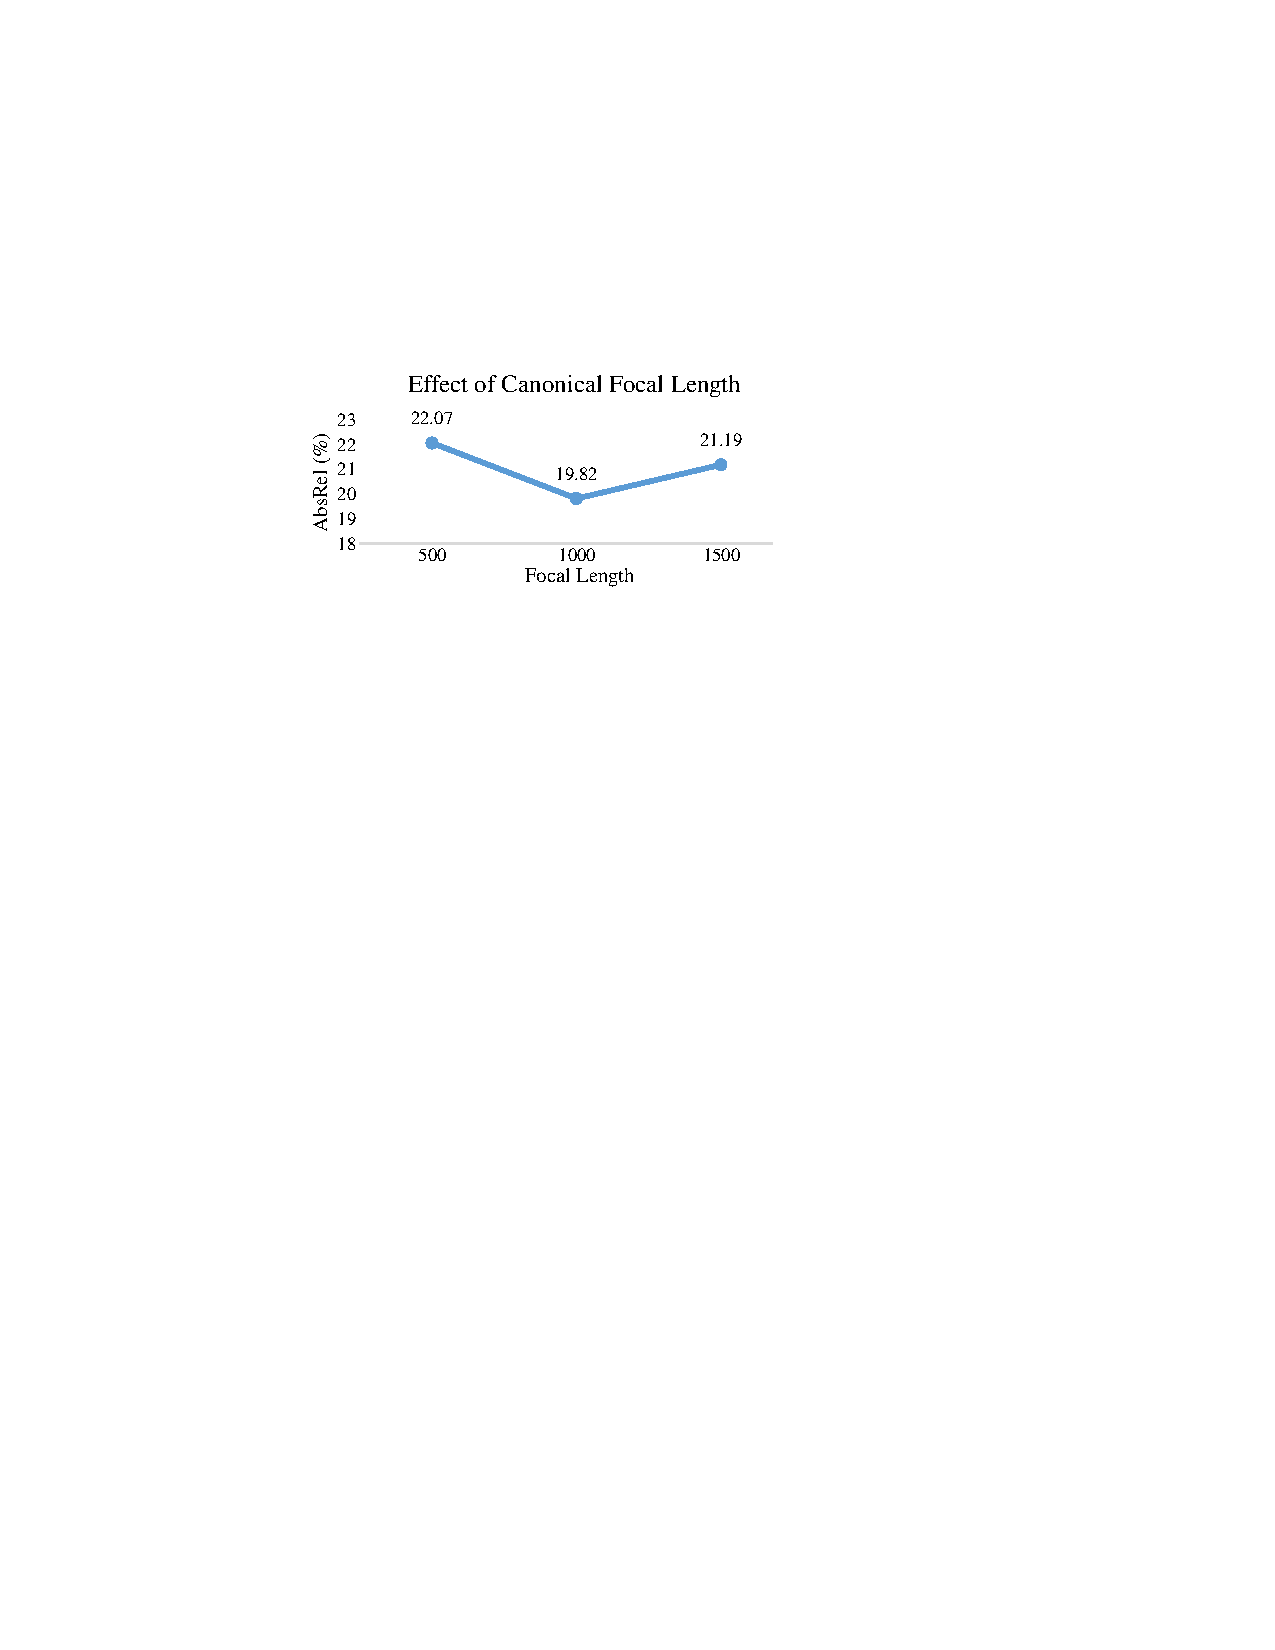
\includegraphics[width=0.3\textwidth]{./files/precision.pdf}
\caption{\textbf{Effect of different canonical focal lengths.} We experiment on different canonical focal lengths and find that too large or small focal lengths will impact the performance. }
\label{fig: canonical focal length.}
\end{figure}

\noindent\textbf{Effectiveness of 
the random proposal normalization loss.}
To show the effectiveness of our proposed random proposal normalization loss (RPNL), we experiment on the sampled small dataset. Results are shown in Tab.~\ref{table: effectiveness of rpnl.}. We test on the DDAD, Lyft, DrivingStereo (DS), NuScenes (NS), KITTI, and NYUv2.  The `baseline' employs all losses except our RPNL. We compare it with `baseline + RPNL' and `baseline + SSIL~\cite{Ranftl2020}'. We can observe that our proposed random proposal normalization loss can further improve the performance. 
In 
contrast, the scale-shift invariant loss~\cite{Ranftl2020}, which does the normalization on the whole image, can only slightly improve the performance. 
\begin{table}[]
\caption{Effectiveness of random proposal normalization loss. Baseline is supervised by `$L_{\PWN} + L_{\VNL} + L_{silog}$'. SSIL is the scale-shift invariant loss proposed in ~\cite{Ranftl2020}.}
\vspace{-1 em}
\scalebox{0.65}{
\begin{tabular}{l|lll|lll}
\toprule[1pt]
\multirow{2}{*}{Method}        & DDAD & Lyft & DS & NS & KITTI & NYUv2 \\ 
        &\multicolumn{3}{c|}{Test set of train. data (AbsRel$\downarrow$)}     & \multicolumn{3}{c}{Zero-shot test set (AbsRel$\downarrow$)} \\  \hline 
baseline  &$0.204$ &$0.251$  &$0.184$  &$0.207$ &$0.104$      &$0.230$     \\
baseline + SSIL~\cite{Ranftl2020} &$0.197$ &$0.263$  &$0.259$  &$0.206$ & $0.105$      &$0.216$     \\
baseline + RPNL   &$\textbf{0.190}$  &$\textbf{0.235}$  &$\textbf{0.182}$  &$\textbf{0.197}$ &$\textbf{0.097}$      &$\textbf{0.210}$     \\  \toprule[1pt]
\end{tabular}}
\label{table: effectiveness of rpnl.}
\vspace{-2 em}
\end{table}



\section{Conclusion} In this paper, we 
tackle 
the problem of reconstructing the 3D metric scene from a single monocular image. To solve the depth ambiguity in image appearance caused by various focal lengths, we propose a canonical camera space transformation method. With our method, we can easily merge millions of data captured by 10k cameras to train one metric depth model. To improve the robustness, we collected over $8$M data for training. Several zero-shot evaluations show the effectiveness and robustness of our work. We further show the ability to do metrology on randomly collected internet images and dense mapping on large-scale scenes. 

\section*{Acknowledgements}

This work was in part supported by National Key R\&D Program of China (No.\  2022ZD0118700).










